\documentclass[xcolor=table, handout]{beamer}

\usepackage{shyne}

% Theme settings
\setbeamertemplate{navigation symbols}{}

\usetheme{Madrid}
\usefonttheme{structurebold}
\usefonttheme[onlymath]{serif}

\AtBeginSection[]
{ 	\begin{frame}{}

	{
	\usebeamerfont{frametitle}
	\begin{beamercolorbox}
		[wd={\textwidth}, center, sep=.2in, rounded=true, shadow=true]
		{frametitle}
	Chapter \thesection\\  \secname 
	\end{beamercolorbox}
	}
	
	\end{frame} 
}

\AtBeginSubsection[]
{ 	\begin{frame}{}

	{
	\usebeamerfont{frametitle}
	\begin{beamercolorbox}
		[wd={\textwidth}, center, sep=.2in, rounded=true, shadow=true]
		{frametitle}
	Section \thesection .\thesubsection\\  \subsecname 
	\end{beamercolorbox}
	}
	
	\end{frame} 
}

\title[Chapter 4]{Stat 201: Statistics I\\ Chapter 4}
\author[M. Shyne]{}
\institute[Metro State]{
\includegraphics[width=1.75in]{../images/metro_logo}}
\date[Sept 18, 2017]{September 18, 2017
\\ \bigskip \bigskip 
\includegraphics[width=.4in]{../images/cc_big}}


\begin{document}
\frame{\titlepage}

% Chapter 4
\setcounter{section}{3}
\section{Probability}

% Section 4.1
\subsection{Basic Concepts of Probability}

\begin{frame}{Terms}
\begin{block}{}
\large A \bt{trial} is conducted to obtain a result from a process with uncertain outcomes. The book also refers to this as a \bt{procedure}.
\end{block}

\pause

\begin{block}{}
\large An \bt{event} is an outcome of interest from a trial.
\end{block}

\pause

\begin{block}{}
\large A \bt{simple event} is an event that cannot be broken down into simpler parts.
\end{block}

\pause

\begin{block}{}
\large A \bt{sample space} is the set of all possible simple events for a trial.
\end{block}
\end{frame}

\begin{frame}{Terms, example}
\begin{exampleblock}{Example}
Consider flipping a coin...
\pause
\begin{itemize}
\item \bt{Trial:} \pause One flip of a coin
\pause
\item \bt{Event:} \pause Getting heads (H)
\pause
\item \bt{Simple event:} \pause This event cannot be broken down, it is a simple event
\pause
\item \bt{Sample space:} \pause Two possible events: \{ H, T \}
\end{itemize}
\end{exampleblock}
\end{frame}

\begin{frame}{Terms, example cont.}
\begin{exampleblock}{Example}
Consider flipping a coin three times...
\begin{itemize}
\pause
\item \bt{Trial:} \pause Three flips of a coin
\pause
\item \bt{Event:} \pause Getting two heads and a tail
\pause
\item \bt{Simple event:} \pause There are several ways this event can occur. It can be broken down into \{ HHT, HTH, THH \}. Getting heads on the first two flips and tails on the third (HHT) is a simple event.
\pause
\item \bt{Sample space:} \pause Eight possible simple events:\\ \{ HHH, HHT, HTH, HTT, THH, THT, TTH, TTT \}
\end{itemize}
\end{exampleblock}

\end{frame}

\begin{frame}{Probability}
\begin{block}{}
{\large \bt{Probability} is a measure of the chance an event will occur in a trial.}
\begin{itemize}
\pause
\item Though sometimes expressed as a percentage, probability is always a number between 0 and 1. 
\pause
\item Probability of 1 means the event is certain to occur and probability of 0 means it is impossible.
\end{itemize}
\end{block}
\pause
\begin{block}{}
Can interpret probability in two ways:
\begin{itemize}
\pause
\item Probability is the proportion an event will occur over a large number of trials. The \bt{law of large numbers} says this proportion will approach the ``true" probability as the number of trials increases.

\pause
\item Some trials can't be repeated (i.e. the weather tomorrow). Then, probability is the level of confidence that an event will occur in a trial (30\% chance of rain tomorrow). 
\end{itemize}
\end{block}
\end{frame}

\begin{frame}{Notation}
\begin{block}{}
Events are designated with capital letters:
\pause
\begin{itemize}
\item $A$ = Get two heads and a tail in three coin flips
\item $B$ = Rain tomorrow
\item $C$ = A randomly selected person is taller than 78 inches
\end{itemize}
\end{block}

\pause
\begin{block}{}
Probabilities are designated with $P()$.
\pause
\begin{itemize}
\item $P(A)$ is the probability of event $A$.
\end{itemize}
\end{block}
\end{frame}

\begin{frame}{Determining probabilities}
\begin{block}{}
\bt{Classical Approach:} If all simple events are equally likely, then
\[P(A) = \frac{\text{number of simple events satisfying } A}{\text{total number of simple events in sample space}}\] 
\end{block}

\pause

\begin{block}{}
\bt{Relative Frequency Approximation:} Given a sample of trials,
\[P(A) = \frac{\text{number of times } A \text{ occured}}{\text{number of trials}}\]
\end{block}

\end{frame}

\begin{frame}{Classical approach, example}
\begin{exampleblock}{Example}
Consider flipping a coin three times. Assuming a fair coin, all simple events are equally likely. Recall the sample space,\\
\smallskip
{\centering
\{ HHH, HHT, HTH, HTT, THH, THT, TTH, TTT \} \par
}
\begin{itemize}
\pause
\item $A$ = Get two heads and a tail, \{ HHT, HTH, THH \}
\pause
\[ P(A) = \frac 3 8\]

\pause
\item $B$ = Get \emph{at least} two heads,  \{ HHH,  HHT, HTH, THH \}
\pause
\[ P(B) = \frac 4 8 = \frac 1 2\]
\end{itemize}
\end{exampleblock}
\end{frame}

\begin{frame}{Relative frequency, example}

\begin{exampleblock}{Example}
The Youth Risk Behavior Survey (YRBS) for 2015 reports that 9421 out of 15624 teenagers surveyed had driven a car at least once in the previous month. Of the 9421 teen drivers, 3806 had texted or emailed while driving. \\
\medskip
What is the probability that a randomly selected teen driver had texted or emailed while driving? 

\pause
\begin{itemize}
\item $A$ = Teen driver has texted or emailed while driving\\
\[P(A) = \frac {3806}{9421} = 0.404\]
\end{itemize}

\end{exampleblock}

\end{frame}


\begin{frame}{Complements}
\begin{block}{}
\large The \bt{comlement} of event $A$, denoted as $\bar A$, consists of all outcomes in the sample space which are not included in $A$.
\end{block}

\pause
\begin{exampleblock}{Example}
\begin{itemize}
\item $A$ = Get a head on one coin flip\\
\pause
$\bar A$ = Get a tail on one coin flip

\pause
\item $B$ = Get exactly two heads on three coin flips\\
\pause
$\bar B$ = Get zero, one or three heads on three coin flips
\end{itemize}
\end{exampleblock}
\end{frame}
 
\begin{frame}{Complement rule }
\begin{block}{}
Since an event and its complement ($A$ and $\bar A$) comprise all possible outcomes, then it is \emph{always} the case that
\[P(A) + P(\bar A) = 1\]
\end{block}

\pause

\begin{exampleblock}{Example}
\begin{itemize}
\item One coin flip: $A$ = \{ H \}, $\bar A$ = \{ T \}
\pause
\[P(A) + P(\bar A) = \frac 1 2 + \frac 1 2 = 1\]

\pause
\item Two heads in three coin flips: $B$ = \{ HHT, HTH, THH \},\\ $\bar B$ = \{ TTT, HTT, THT, TTH, HHH \}
\pause
\[P(B) + P(\bar B) = \frac 3 8 + \frac 5 8 = 1\]
\end{itemize}
\end{exampleblock}
\end{frame}

\begin{frame}{Using the complement rule}
\begin{exampleblock}{}
The Youth Risk Behavior Survey (YRBS) for 2015 reports that 9421 out of 15624 teenagers surveyed had driven a car at least once in the previous month. Of the 9421 teen drivers, 3806 had texted or emailed while driving. \\
\medskip
What is the probability that a randomly selected teen driver had \emph{not} texted or emailed while driving? 

\begin{itemize}
\pause
\item $A$ = Teen driver has texted or emailed while driving\\
$\bar A$ = Teen driver has not texted or emailed while driving
\pause
\item \[P(A) = \frac {3806}{9421} = 0.404\]
\vspace*{-\baselineskip}\pause
\item \[P(\bar A) = 1 - P(A) = 1 - 0.404 = 0.596 \]
\end{itemize}
\end{exampleblock}
\end{frame}

\begin{frame}{Unlikely vs. unusual events}
\begin{block}{}
\large An event is \bt{unlikely} if its probability is below some threshold,\\ usually 0.05.
\end{block}

\begin{block}{}
\large An event is \bt{unusual} if it represents an extreme outcome.
\end{block}

\pause

\begin{exampleblock}{Example}
Consider flipping a fair coin 1000 times. Expect heads half of the time, for a total of 500.

\begin{itemize}
\pause
\item Let $A$ be the event of exactly 523 heads.
\begin{itemize}
\pause
\item $A$ is unlikely ($P(A) = 0.00876$), but not unusual.
\end{itemize}

\pause
\item  Let $B$ be the event of exactly 46 heads.
\begin{itemize}
\pause
\item $B$ is very unlikely ($P(B) = 5.929 \times 10^{-222}$) and unusual.
\end{itemize}
\end{itemize}
\end{exampleblock}
\end{frame}

\begin{frame}{Practice: Cancer screening}
\begin{block}{}
Suppose a company is testing a new, cheaper screening test for cancer. They gather a random sample, giving every subject the new test and a doctor visit for definitive diagnosis. These are the results.\\
\medskip
{\centering
\begin{tabular}{c | c  c}
\multicolumn{1}{c}{} & \multicolumn{2}{c}{Test Result}\\
Diagnosis & Positive & Negative\\
\hline
Cancer & 74 & 13\\
No cancer & 26 & 887 \\
\end{tabular}\par
}
\smallskip
\begin{itemize}
\pause
\item The number 26 represents \bt{false positives}, positive test results for those with no cancer.
\pause
\item The number 13 represents \bt{false negatives}, negative test results for those with cancer.
\end{itemize}
\end{block}
\end{frame}

\begin{frame}{Practice: Cancer screening, cont.}
\begin{block}{}
{\centering
\begin{tabular}{c | c  c }
\multicolumn{1}{c}{} & \multicolumn{2}{c}{Test Result}\\
Diagnosis & Positive & Negative \\
\hline
Cancer & 74 & 13 \\
No cancer & 26 & 887\\
\end{tabular}\par
}
\end{block}

\begin{exampleblock}{}
What is the probability of a randomly selected person having cancer?
\begin{itemize}
\pause
\item \[P(\text{cancer}) = \frac {74 + 13}{74+13+26+887} = \frac {87}{1000} = 0.087\]
\end{itemize}

\pause
What is the probability of a false negative (person has cancer, but test result is negative)?
\begin{itemize}
\pause
\item \[ P(\text{false negative}) = \frac {13}{1000} = 0.013\]
\end{itemize}
\end{exampleblock}
\end{frame}

\begin{frame}<handout:0>{Group work}
\begin{block}{}
\large
\begin{itemize}
\item For questions 1 through 3, complete part (a).
\item Probabilities can be expressed as fractions.
\end{itemize}
\end{block}
\end{frame}

% Section 4.2
\subsection{Addition Rule and Multiplication Rule}

\begin{frame}{Compound events}
\begin{block}{}
{\large A \bt{compound event} is an event which occurs when at least one of two or more simple events occur. }
\begin{itemize}
\pause
\item Denoted as $C = A$ \bt{or} $B$
\end{itemize}
\end{block}

\begin{exampleblock}{Example}
\begin{itemize}
\item $A$ = Get exactly two heads in three flips\\
$A$ = HHT or HTH or THH

\pause
\item $A$ = Student gets an A on midterm\\
$B$ = Student gets a B on midterm\\
$C$ = A or B = Student gets an A or a B on midterm

\pause
\item $A$ = Student gets an A on midterm\\
$B$ = Student is female\\
$C$ = A or B = Student gets an A on midterm or is female
\end{itemize}
\end{exampleblock}
\end{frame}

\begin{frame}{Disjoint events}
\begin{block}{}
\bt{Disjoint events} are two (or more) events that cannot occur simultaneously. Also called \bt{mutually exclusive}.
\begin{itemize}
\pause
\item Complements are always disjoint.
\end{itemize}
\end{block}

\begin{exampleblock}{Example}
\begin{itemize}
\item $A$ = Get exactly two heads in three flips\\
$B$ = Get exactly zero, one or three heads in three flips\\
\pause
$A$ and $B$ are complements, thus they are disjoint.

\pause
\item $A$ = Student gets an A on midterm\\
$B$ = Student gets a B on midterm\\
\pause
$A$ and $B$ are disjoint, cannot get an A and a B on the midterm

\pause
\item $A$ = Student gets an A on midterm\\
$B$ = Student is female\\
\pause
$A$ and $B$ are \emph{not} disjoint, possible to get an A and be female
\end{itemize}

\end{exampleblock}
\end{frame}

\begin{frame}{Venn diagrams}
\begin{block}{}
\large \bt{Venn diagrams} are a good way to visualize events in a sample space.
\end{block}
{\centering
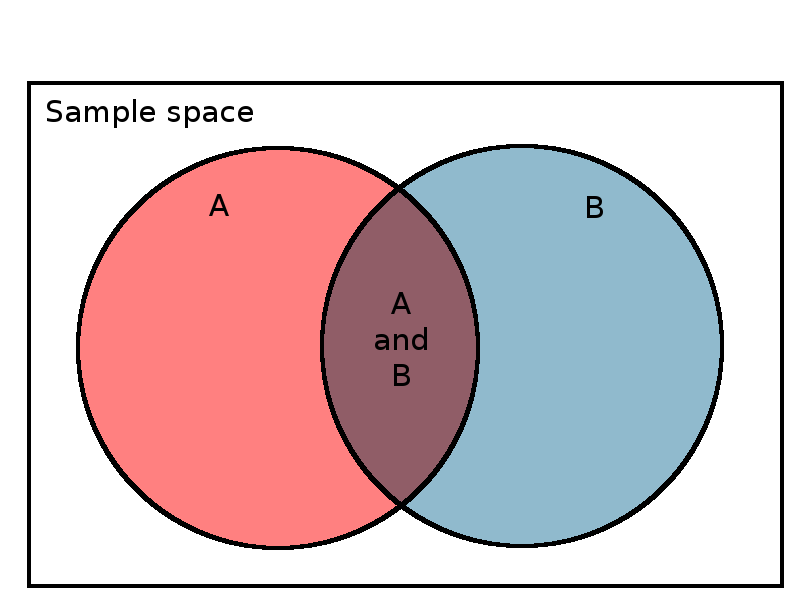
\includegraphics[width=3in]{../images/ch4_venn_ovr}\par
}
\end{frame}

\begin{frame}{Venn diagrams, disjoint events}
\begin{block}{}
\large Disjoint events are represented non-overlapping circles.
\end{block}
{\centering
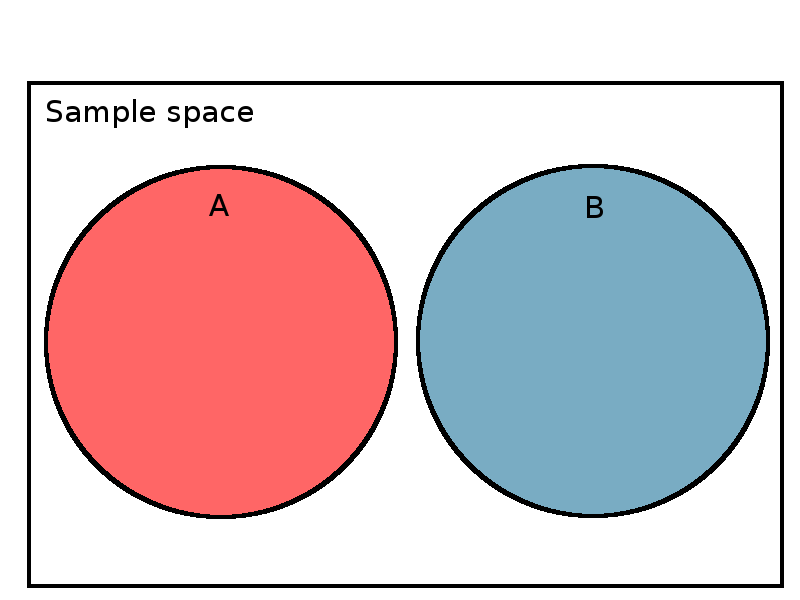
\includegraphics[width=3in]{../images/ch4_venn_dsj}\par
}
\end{frame}

\begin{frame}{Venn diagrams, complements}
\begin{block}{}
\large Complements are the whole sample space except the event area.
\end{block}
{\centering
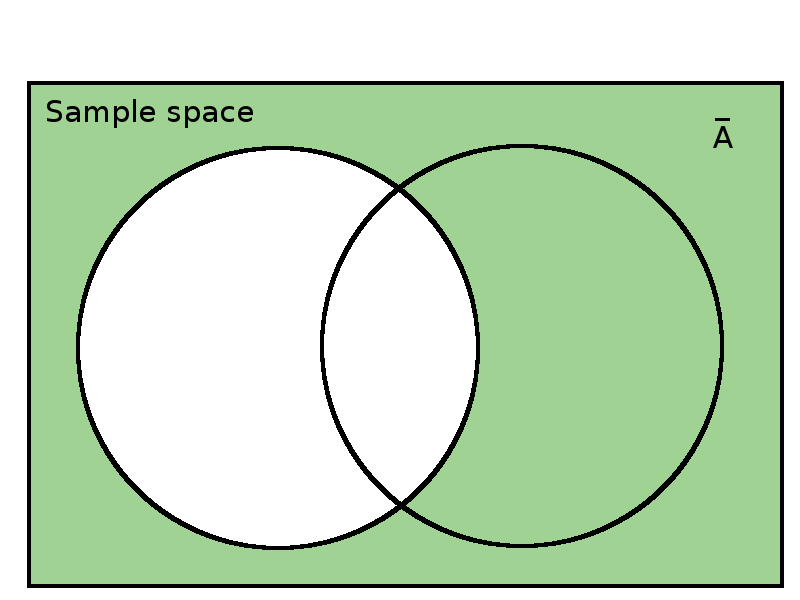
\includegraphics[width=3in]{../images/ch4_venn_a_comp}\par
}
\end{frame}

\begin{frame}{Addition rule}
\begin{block}{}
The general rule for calculating probabilities of compound events is to count the outcomes satisfying A and the outcomes satisfying B, making sure to only count each outcome once, and then divide by total number of outcomes.
\end{block}

\pause
\begin{block}{}
The formal rule is
\[P(A \text{ or } B) = P(A) + P(B) - P(A \text{ and } B)\]

\pause
For disjoint events, $P(A \text{ and } B) = 0$, so the rule becomes,
\[P(A \text{ or } B) = P(A) + P(B)\]
\end{block}
\end{frame}

\begin{frame}{Addition rule, example}
\begin{block}{}
Suppose a statistics class has 100 students. On the midterm, 40 students got an A (event $A$) and 30 students got a B (event $B$).
\end{block}

{\centering
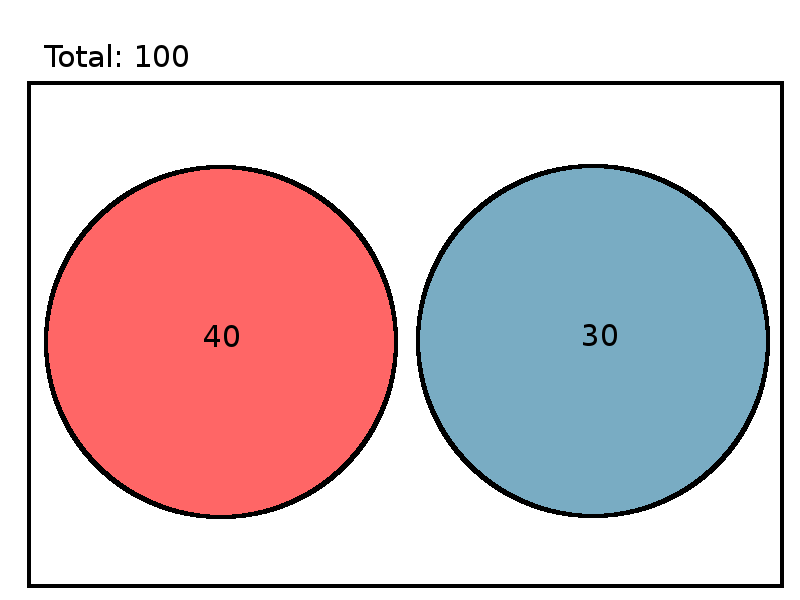
\includegraphics[width=3in]{../images/ch4_venn_dsj_ex}\par
}
\end{frame}

\begin{frame}{Addition rule, example cont.}
\begin{block}{}
Suppose a statistics class has 100 students. On the midterm, 40 students got an A (event $A$) and 30 students got a B (event $B$).
\end{block}

\begin{exampleblock}{}
What is the probability that a randomly selected student got an A or a B?
\begin{itemize}
\pause
\item By the general rule, 40 outcomes for event $A$ and 30 outcomes for event $B$, and none are counted twice. So,
\[P(A \text{ or } B) = \frac {40 + 30}{100} = 0.7\]
\pause
\item By the formal rule, $P(A \text{ or } B) = P(A) + P(B) - P(A \text{ and } B)$.
\[P(A) = 0.4 \qquad P(B) = 0.3 \qquad P(A \text{ and } B) = 0\]
\[P(A \text{ or } B) = 0.4 + 0.3 - 0 = 0.7\]

\end{itemize}
\end{exampleblock}
\end{frame}

\begin{frame}{Addition rule, example 2}
\begin{block}{}
Suppose a statistics class has 100 students. On the midterm, 40 students got an A (event $A$),  70 students are female (event $B$) and 25 of the female students got an A.
\end{block}

{\centering
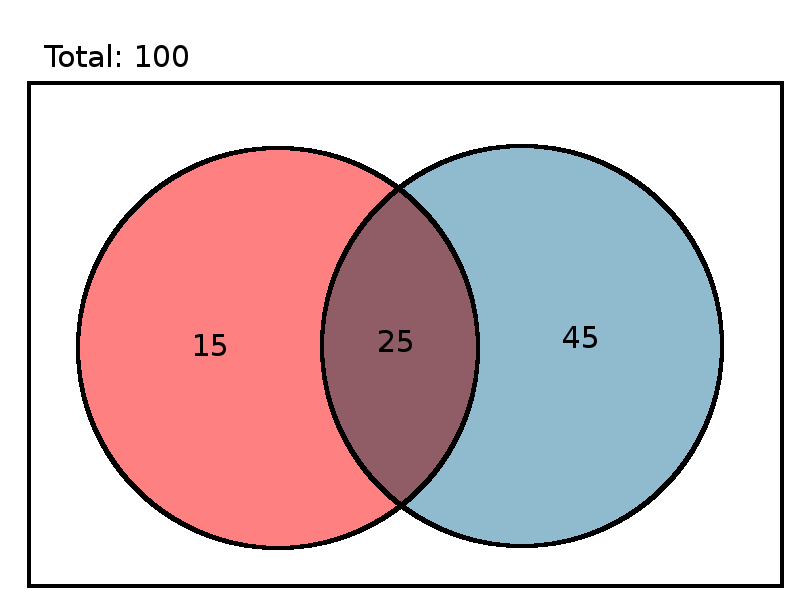
\includegraphics[width=3in]{../images/ch4_venn_ovr_ex}\par
}
\end{frame}

\begin{frame}{Addition rule, example 2 cont.}
\begin{block}{}
Suppose a statistics class has 100 students. On the midterm, 40 students got an A (event $A$),  70 students are female (event $B$) and 25 of the female students got an A.
\end{block}
\begin{exampleblock}{}
What is the probability that a randomly selected student got an A or is female?
\begin{itemize}
\pause
\item By the general rule, if outcomes were counted as in the previous example,
\[P(A \text{ or } B) = \frac {40 + 70}{100} = 1.1\]

\pause
\item The females who got A's were counted twice. Instead, count distinct outcomes in the circles of the Venn diagram.
\[P(A \text{ or } B) = \frac {15 + 25 + 45}{100} = 0.85\]

\end{itemize}
\end{exampleblock}

\end{frame}

\begin{frame}{Addition rule, example 2 cont.}
\begin{block}{}
Suppose a statistics class has 100 students. On the midterm, 40 students got an A (event $A$),  70 students are female (event $B$) and 25 of the female students got an A.
\end{block}

\begin{exampleblock}{}
What is the probability that a randomly selected student got an A or is female?
\begin{itemize}
\pause
\item By the formal rule, $P(A \text{ or } B) = P(A) + P(B) - P(A \text{ and } B)$.
\[P(A) = 0.4 \qquad P(B) = 0.7 \qquad P(A \text{ and } B) = 0.25\]
\[P(A \text{ or } B) = 0.4 + 0.7 - 0.25 = 0.85\]
\end{itemize}
\end{exampleblock}
\end{frame}

\begin{frame}{Addition rule, example 2 table}
\begin{block}{}
Suppose a statistics class has 100 students. On the midterm, 40 students got an A (event $A$),  70 students are female (event $B$) and 25 of the female students got an A.
\end{block}

\begin{exampleblock}{}
Construct a table for this situation.\\
\pause
\medskip
{\centering
\begin{tabular}{c | c  c | c}
\multicolumn{1}{c}{} & \multicolumn{2}{c}{Midterm grade}\\
Gender & A & Not A & Total\\
\hline
Female & 25 & 45 & 70\\
Male & 15 & 15 & 30 \\
\hline
Total & 40 & 60 & 100
\end{tabular}\par
}
\end{exampleblock}
\end{frame}

\begin{frame}{Complements, revisited}
\begin{block}{}
Remember, an event and its complement comprise the whole sample space. Whatever the result of a trial, it satisfies either the event or its complement.
\[P(A \text{ or } \bar A) = 1 \]
\pause
Also, complements are disjoint, so the addition rule is
\[P(A \text{ or } \bar A) = P(A) + P(\bar A) \]
\pause
Then,
\[P(A) + P(\bar A) = 1 \]
\[P(A) = 1 -  P(\bar A) \]
\[P(\bar A) = 1 - P(A) \]


\end{block}
\end{frame}

\begin{frame}{Practice: Cancer screening}
\begin{block}{}
{\centering
\begin{tabular}{c | c  c | c}
\multicolumn{1}{c}{} & \multicolumn{2}{c}{Test Result}\\
Diagnosis & Positive & Negative & Total \\
\hline
Cancer & 74 & 13 & 87\\
No cancer & 26 & 887 & 913\\
\hline
Total & 100 & 900 & 1000
\end{tabular}\par
}
\end{block}

\begin{exampleblock}{}
What is the probability of a randomly selected person having cancer ($A$) or not having cancer ($B$)?

\begin{itemize}
\pause
\item Having cancer and not having cancer are complements,
\[ P(A \text{ or } B) = 1\]
\end{itemize}
\end{exampleblock}
\end{frame}

\begin{frame}{Practice: Cancer screening, cont.}
\begin{block}{}
{\centering
\begin{tabular}{c | c  c | c}
\multicolumn{1}{c}{} & \multicolumn{2}{c}{Test Result}\\
Diagnosis & Positive & Negative & Total \\
\hline
Cancer & 74 (0.074) & 13 (0.013) & 87 (0.087)\\
No cancer & 26 (0.026) & 887 (0.887) & 913 (0.913)\\
\hline
Total & 100 (0.1) & 900 (0.9) & 1000 (1)
\end{tabular}\par
}
\end{block}

\begin{exampleblock}{}
What is the probability of a randomly selected person having cancer ($A$) or getting a positive test result ($B$)?

\begin{itemize}
\pause
\item Using the addition rule,
\[ P(A \text{ or } B) = 0.087 + 0.1 - 0.074 = 0.113\]
\end{itemize}
\end{exampleblock}
\end{frame}

\begin{frame}{Practice: Cancer screening, cont.}
\begin{block}{}
{\centering
\begin{tabular}{c | c  c | c}
\multicolumn{1}{c}{} & \multicolumn{2}{c}{Test Result}\\
Diagnosis & Positive & Negative & Total \\
\hline
Cancer & 74 (0.074) & 13 (0.013) & 87 (0.087)\\
No cancer & 26 (0.026) & 887 (0.887) & 913 (0.913)\\
\hline
Total & 100 (0.1) & 900 (0.9) & 1000 (1)
\end{tabular}\par
}
\end{block}

\begin{exampleblock}{}
What is the probability of a test being wrong? That is, what is the probability of getting a false positive ($A$) or a false negative ($B$)?

\begin{itemize}
\pause
\item The events are disjoint. Using simplified addition rule,
\[ P(A \text{ or } B) = 0.026 + 0.013 = 0.039\]
\end{itemize}
\end{exampleblock}
\end{frame}

\begin{frame}<handout:0>{Group work}
\begin{block}{}
\large
\begin{itemize}
\item For questions 1 through 3, complete part (b).
\item Probabilities can be expressed as fractions.
\end{itemize}
\end{block}
\end{frame}


\begin{frame}{Independent events}
\begin{block}{}
\large Two events are said to be \bt{independent} if the probability of one is unaffected by the occurrence of the other.
\end{block}

\pause

\begin{exampleblock}{Example}
\begin{itemize}
\item Let $A$ = get a head on the first flip\\
and $B$ = get a tail on the second flip.\\
$P(B) = \frac 1 2$ regardless of what happens on the first flip.
\end{itemize}
\end{exampleblock}
\end{frame}

\begin{frame}{Dependent events}
\begin{block}{}
\large If two events are not independent, then they are \bt{dependent}. That is, the probability of one changes depending on the outcome of the other.
\end{block}

\pause

\begin{exampleblock}{Example}
Consider an urn with 2 red balls and 3 blue balls. A trial consists of randomly selecting a ball from the urn and not replacing it.\\
\pause
\begin{itemize}
\item Let $A$ = get a red ball the first trial\\
 and $B$ = get a blue ball the second trial.
\begin{itemize}
\pause
\item If $A$ occurs, then $P(B) = 3 / 4$
\pause
\item If $A$ does not occur, then $P(B) =  2 / 4$
\end{itemize}
\end{itemize}
\end{exampleblock}

\pause

\begin{exampleblock}{Example}
The probability of a randomly selected student getting an A on the final is probably different depending on whether they got an A on the midterm.
\end{exampleblock}
\end{frame}

\begin{frame}{Dependent events as independent}
\begin{block}{}
When dealing with large populations and small sample sizes, events that are technically dependent can be treated as independent. The rule of thumb the book uses is sample sizes less than 5\% of population can be treated as independent.
\end{block}

\pause
\begin{exampleblock}{Example}
Suppose the urn has 2000 red balls and 3000 blue balls. The probability of selecting a blue ball is approximately $3/5$, regardless of whether a red ball was previously selected or not.
\end{exampleblock}
\end{frame}

\begin{frame}{Conditional probability}
\begin{block}{}
\large The \bt{conditional probability} of an event is the probability assuming another event occurred. 
\begin{itemize}
\pause
\item It is denoted $P(B|A)$ and read as ``probability of $B$ given $A$"
\pause
\item For independent events, $P(B|A) = P(B)$
\end{itemize}
\end{block}

\pause

\begin{exampleblock}{Example}
There is an urn with 2 red balls and three blue balls. A trial consists of randomly selecting a ball from the urn and not replacing it.\\
Let $A$ = get a red ball the first trial\\
 and $B$ = get a blue ball the second trial.
\begin{itemize}
\pause
\item $P(B | A) = 3 / 4$
\pause
\item $P(B | \bar A) =  2 / 4$
\end{itemize}

\end{exampleblock}
\end{frame}

\begin{frame}{Multiplication rule}
\begin{block}{}
To find the probability of all events in a series of trials, multiply the probability of the first by the probability of the second given the first occurred, etc.\\
\medskip
\pause
Formally,
\[P(A \text{ and } B) = P(A) \times P(B|A)\]
\pause
For independent events,
\[P(A \text{ and } B) = P(A) \times P(B)\]
\end{block}
\end{frame}

\begin{frame}{Multiplication rule, example}
\begin{exampleblock}{Example}
There is an urn with 2 red balls and 3 blue balls. A trial consists of randomly selecting a ball from the urn and not replacing it.\\
\medskip 
What is the probability of selecting a red ball and then selecting a blue ball?
\begin{itemize}
\pause
\item Let $A$ = get a red ball the first trial\\
 and $B$ = get a blue ball the second trial.\\

\pause
\item $B$ is dependent on $A$.
\[P(A \text{ and } B) = P(A) \times P(B|A)\]

\pause
\item $P(A) = 2/5 \qquad P(B|A) = 3/4$

\pause
\item
\[P(A \text{ and } B) = \frac 2 5 \times \frac 3 4 = \frac 6 {20} = \frac 3 {10} = 0.3\]

\end{itemize}

\end{exampleblock}
\end{frame}

\begin{frame}{Multiplication rule, example}
\begin{exampleblock}{Example}
Consider flipping a coin three times.\\
\medskip 
What is the probability of get heads on the first two flips and a tail on the third (HHT)?
\begin{itemize}
\pause
\item Let $A$ = get a head the first flip,\\
 $B$ = get a head on the second flip,\\
and $C$ = get a tail on the third flip.

\pause
\item $A$, $B$ and $C$ are independent events. 
\[P(A \text{ and } B \text{ and } C) = P(A) \times P(B) \times P(C)\]

\pause
\item $P(A) = P(B) = P(C) = 1/2$

\pause
\item
\[P(A \text{ and } B \text{ and } C) = \frac 1 2 \times \frac 1 2 \times \frac 1 2 = \frac 1 8\]

\end{itemize}

\end{exampleblock}
\end{frame}

\begin{frame}{Tree diagrams}
\begin{block}{}
\large \bt{Tree diagrams} are a good way to visualize events in a series of trials.
\end{block}
\bigskip
{\centering
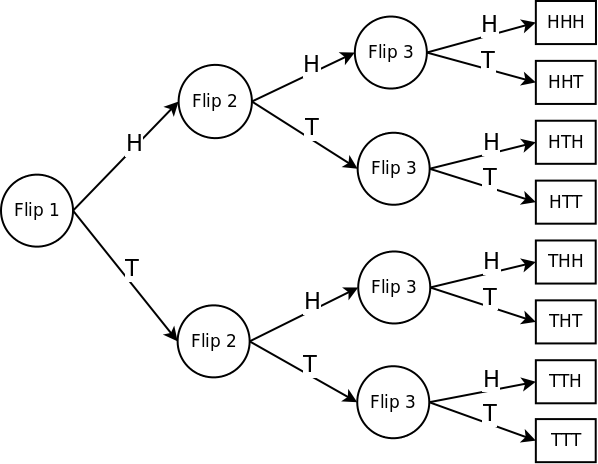
\includegraphics[width=3in]{../images/tree_diagram_coin}\par
}
\end{frame}

\begin{frame}{Tree diagram, urn example}

{\centering
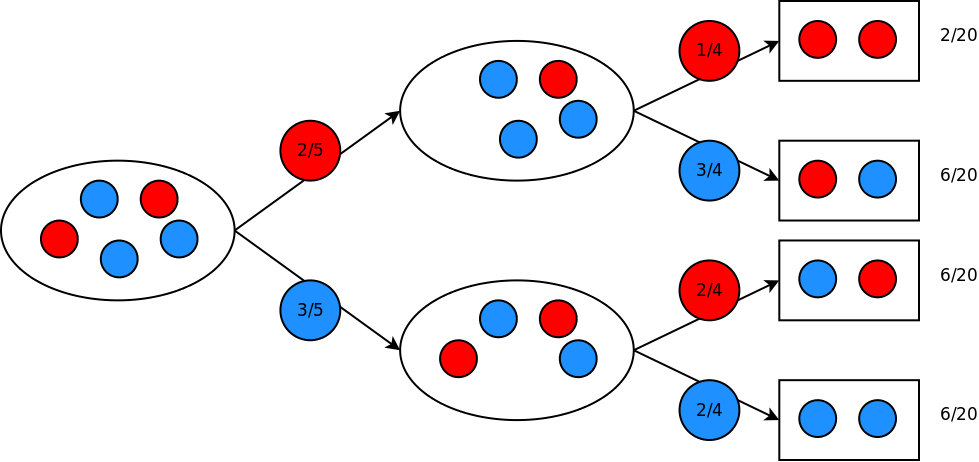
\includegraphics[width=4in]{../images/tree_diagram_balls}\par
}
\end{frame}

\begin{frame}{Practice: Cancer screening}
\begin{block}{}
{\centering
\begin{tabular}{c | c  c | c}
\multicolumn{1}{c}{} & \multicolumn{2}{c}{Test Result}\\
Diagnosis & Positive & Negative & Total \\
\hline
Cancer & 74 & 13 & 87\\
No cancer & 26 & 887 & 913\\
\hline
Total & 100 & 900 & 1000
\end{tabular}\par
}
\end{block}

\begin{exampleblock}{}
What is the probability of two randomly selected people both having positive test results?

\begin{itemize}
\pause
\item Sample size of 2 is less than 5\% of population of 1000, so can treat events as independent.
\pause
\item $P(\text{positive}) = \frac {100}{1000} = 0.1$
\pause
\item $P(\text{both positive}) = 0.1 \times 0.1 = 0.01$
\end{itemize}
\end{exampleblock}

\end{frame}

\begin{frame}{Practice: Statistics club}
\begin{block}{}
The Metro State Statistics Club has 10 members, 6 men and 4 women. They need to select a president, a vice-president and a treasurer. They decide to choose members randomly for the officers positions, in order.
\end{block}
\pause
\begin{exampleblock}{}
What is the probability that women are selected for president and vice-president, and a man for treasurer?
\begin{itemize}
\pause
\item $A$ = Woman selected president\\
$B$ = Woman selected vice-president\\
$C$ = Man selected treasurer
\pause
\item $P(A \text{ and } B \text{ and } C) = P(A) \times P(B|A) \times P(C | A \text{ and } B)$\\
\pause
\item $P(A) = \frac 4{10} = 0.4$\\
$P(B|A) = \frac 3 9 = 0.33$\\
$P(C | A \text{ and } B) = \frac 6 8 = .75$

\pause
\item $P(A \text{ and } B \text{ and } C) = 0.4 \times 0.33 \times 0.75 = 0.099$ 
\end{itemize}
\end{exampleblock}
\end{frame}

\begin{frame}{Recap of probability rules}
\begin{block}{}
\begin{itemize}
\item To calculate the probability of at least one of two events occurring\\ ($A$ \bt{or} $B$), use the addition rule. Be aware of whether the events are disjoint or not.

\pause
\item To calculate  the probability of all of a sequence of two, or more, events occurring ($A$ \bt{and} $B$), use the multiplication rule. Be aware of whether the events are independent or dependent.
\end{itemize}
\end{block}
\end{frame}

\begin{frame}{Testing for independence}
\begin{block}{}
It is sometimes difficult to tell if events are independent. The rule for independent events, that $P(B|A) = P(B)$, can be used to test for independence.
\end{block}
\end{frame}

\begin{frame}{Testing for independence, example}
\begin{exampleblock}{Example}
Consider rolling two fair six-sided dice. Let $A$ = total of the dice is 5 and $B$ = at least one of the dice is a 3.\\
\medskip
Are $A$ and $B$ independent events?
\begin{itemize}
\pause
\item $P(B) = P(\text{first die is 3 or second die is 3}) $\\
$P(B) = P(\text{first die is 3}) + P(\text{second die is 3}) - P(\text{both are 3}) $\\
$P(B) = \frac 1 6 + \frac 1 6 - \frac 1 {36} = \frac {11}{36}$
\pause
\item If $A$ occurred, then the possible dice values are\\ 
{\centering $\set{(1,4), (2,3), (3,2), (4,1)}$\par }

\pause
\item $P(B|A) = \frac 2 4 = \frac 1 2$

\pause
\item $A$ and $B$ are not independent.
\end{itemize} 
\end{exampleblock}
\end{frame}

\begin{frame}<handout:0>{Group work}
\begin{block}{}
\large
\begin{itemize}
\item For questions 1 through 3, complete part (c).
\item Probabilities can be expressed as fractions.
\end{itemize}
\end{block}
\end{frame}

% Section 4.3
\subsection{Complements, Conditional Probability and Bayes' Theorem}

\begin{frame}{Complex events}

\begin{block}{}
{\large A \bt{complex event} is a compound event in the form of ``at least one" of some simpler event occurs.}
\begin{itemize}
\pause
\item This is a shortcut for ``exactly one \bt{or} exactly two \bt{or}..."
\end{itemize}
\end{block}

\pause

\begin{block}{}
The complement of a complex event is none of the simpler events occur, or that the simpler event didn't occur all the time.
\end{block}

\begin{exampleblock}{Example}
Let $A$ = Get at least one head in three flips.
\begin{itemize}
\pause
\item $A$ = exactly one head \bt{or} exactly two heads \bt{or} exactly three heads
\pause
\item $\bar A$ = Get no heads on three flips = Get tails every flip
\end{itemize}
\end{exampleblock}
\end{frame}

\begin{frame}{Using complements for complex events}
\begin{block}{}
As sample sizes increases, calculating probabilities for complex events becomes very difficult. It is often much easier to use complements for such calculations.

\begin{itemize}
\item Recall the complement rule,
\[P(A) = 1 - P(\bar A)\]
\end{itemize}
\end{block}
\end{frame}

\begin{frame}{Using complements for complex events, example}
\begin{exampleblock}{Example}
A manufacturer of insulin test strips has a defect rate of 0.7\% ($P(\text{strip is defective}) = 0.007$). In a box a 50 strips, what is the probability of getting at least one defective strip?
\begin{itemize}
\pause
\item $A$ = At least one strip is defective\\
$\bar A$ = No strips are defective = All strips are good
\pause
\item $P(\text{strip is good}) = 1 - P(\text{strip is defective}) = 1 - 0.007 = 0.993$ 
\pause
\item \[P(\bar A) = 0.993 \times 0.993 \times \cdots \times 0.993\]
\[P(\bar A) = (0.993)^{50} = 0.704\]
\vspace*{-\baselineskip}\pause 
\item \[P(A) = 1 - P(\bar A) = 1 - 0.704 = 0.296\]
\end{itemize}
\end{exampleblock}
\end{frame}

\begin{frame}{Other kinds of complex events}
\begin{block}{}
A complex event could be in the form of ``at least twice" or "at least three times", etc.\\
\medskip
\pause
The complements in these cases, ``the event occurs zero or one times", is still probably simpler to calculate.
\end{block}
\end{frame}

\begin{frame}{Practice: cancer screening}
\begin{block}{}
{\centering \renewcommand{\arraystretch}{1}
\begin{tabular}{c | c  c | c}
 & Positive & Negative & Total \\
\hline
Cancer & 74 (0.074) & 13 (0.013) & 87 (0.087)\\
No cancer & 26 (0.026) & 887 (0.887) & 913 (0.913)\\
\hline
Total & 100 (0.1) & 900 (0.9) & 1000 (1)
\end{tabular}\par
\renewcommand{\arraystretch}{1.5}
}
\end{block}

\begin{exampleblock}{}
If ten subjects are selected randomly, what is the probability at least one of them test positive?
\begin{itemize}
\pause
\item $A$ = At least one test positive\\
$\bar A$ = Zero test positive = All test negative
\pause
\item  
\[P(\bar A) = (0.9)^{10} = 0.349\]
\vspace*{-\baselineskip}\pause
\item  
\[P(A) = 1 - 0.349  = 0.651\]
\end{itemize}
\end{exampleblock}

\end{frame}

\begin{frame}{Formal definition of conditional probability}

\begin{block}{}
Recall the multiplication rule,
\[P(A \text{ and } B) = P(A) \times P(B|A)\]
\pause
From this, the formal definition of conditional probability is
\[P(B|A) = \frac {P(A \text{ and } B)}{P(A)}\] 
\end{block}
\end{frame}

\begin{frame}{Intuitive approach to conditional probability}

\begin{block}{}
An intuitive approach to $P(B|A)$ is to assume $A$ has occurred, then count count instances of $B$. $A$ is, in a sense, the new sample space.
\[ P(B|A) = \frac{\text{number of $B$ and $A$}}{\text{number of $A$}}\]
\end{block}
\end{frame}

\begin{frame}{Practice: Cancer screening}
\begin{block}{}
{\centering \renewcommand{\arraystretch}{1}
\begin{tabular}{c | c  c | c}
 & Positive & Negative & Total \\
\hline
Cancer & 74 (0.074) & 13 (0.013) & 87 (0.087)\\
No cancer & 26 (0.026) & 887 (0.887) & 913 (0.913)\\
\end{tabular}\par
\renewcommand{\arraystretch}{1.5}
}
\end{block}

\begin{exampleblock}{}
What is the probability of a positive test result if the subject has cancer?
\begin{itemize}
\pause
\item $A$ = Subject has cancer\\
$B$ = Positive test result
\pause
\item Formally,
\[P(B|A) = \frac {P(A \text{ and } B)}{P(A)} = \frac {0.074}{0.087} = 0.851\]
\vspace*{-\baselineskip}\pause
\item Intuitive approach,
\[ P(B|A) = \frac{\text{number of $B$ and $A$}}{\text{number of $A$}} = \frac {74}{87} = 0.851\]
\end{itemize}
\end{exampleblock}
\end{frame}

\begin{frame}{Practice: Cancer screening, cont.}
\begin{block}{}
{\centering \renewcommand{\arraystretch}{1}
\begin{tabular}{c | c  c | c}
 & Positive & Negative & Total \\
\hline
Cancer & 74 (0.074) & 13 (0.013) & 87 (0.087)\\
No cancer & 26 (0.026) & 887 (0.887) & 913 (0.913)\\
\end{tabular}\par
\renewcommand{\arraystretch}{1.5}
}
\end{block}

\begin{exampleblock}{}
What is the probability of a negative test result if the subject does not have cancer?
\begin{itemize}
\pause
\item $A$ = Subject does not have cancer\\
$B$ = Negative test result
\pause
\item Formally,
\[P(B|A) = \frac {P(A \text{ and } B)}{P(A)} = \frac {0.887}{0.913} = 0.972\]
\vspace*{-\baselineskip}\pause
\item Intuitive approach,
\[ P(B|A) = \frac{\text{number of $B$ and $A$}}{\text{number of $A$}} = \frac {887}{913} = 0.972\]
\end{itemize}
\end{exampleblock}
\end{frame}

\begin{frame}{Sensitivity and specificity}
\begin{block}{}
The proceeding examples have specific terms when used with diagnostic tests.
\begin{itemize}
\pause
\item \bt{Sensitivity} is the probability of a positive test result for a subject which has the conditions, $P(\text{positive}|\text{cancer})$.
\pause
\item \bt{Specificty} is the probability of a negative test result for a subject which does not have the conditions, $P(\text{negative}|\text{no cancer})$.
\end{itemize}

\pause
Many diagnostic tests work by measuring the level of a certain chemical and returning a positive result if it is above a designated threshold. Adjusting this threshold to increase sensitivity will decrease specificity, and vice versa. There is always a trade-off.
\end{block}
\end{frame}

\begin{frame}{Screening tests for rare events}
\begin{exampleblock}{Example}
Suppose there is a screening test for a rare disease which has a prevalence of 0.3\%. The screening test has 99\% sensitivity and 99\% specificity. 100,000 people are screened.\\
\smallskip
{\centering \renewcommand{\arraystretch}{1}
\begin{tabular}{c | c  c | c}
 & Positive & Negative & Total \\
\hline
Disease & 297 & 3 & 300\\
No disease & 997 & 98703 & 99700\\
\hline
Total & 1294 & 98706 & 100,000 
\end{tabular}\par
\renewcommand{\arraystretch}{1.5}
}
\smallskip
What is the probability that someone who tested positive does not have the disease?
\begin{itemize}
\pause
\item \[P(\text{no disease} | \text{positive}) = \frac {997}{1294} = 0.770\]
\vspace*{-\baselineskip}\pause
\item The complement, $P(\text{disease} | \text{positive}) = 0.23$, is known as the \bt{precision} or the \bt{positive predictive value (PPV)} of the test.
\end{itemize}

\end{exampleblock}
\end{frame}

\begin{frame}{Screening tests for rare events, cont.}
\begin{block}{}
\begin{itemize}
\item This does not mean screening tests are not useful. Often they are a first step before tests that are more accurate, but also more expensive and/or more invasive.
\begin{itemize}
\item Cancer screening, followed by biopsy for confirmation
\end{itemize}

\pause
\item Sometimes tests like these can have profound consequences for peoples lives.
\begin{itemize}
\item Drug screening for jobs
\item Vetting for refugees or immigrants 
\item etc.
\end{itemize}

\pause
\item It is important to remember that no test is perfect and there are often trade-offs (sensitivity / specificity).
\end{itemize}
\end{block}
\end{frame}

\begin{frame}<handout:0>{Group work}
\begin{block}{}
\large
\begin{itemize}
\item Complete question 4.
\item Probabilities can be expressed as fractions.
\end{itemize}
\end{block}
\end{frame}

\end{document}